% Options for packages loaded elsewhere
\PassOptionsToPackage{unicode}{hyperref}
\PassOptionsToPackage{hyphens}{url}
%
\documentclass[
  12pt,
  a4paper,
  DIV=11,
  numbers=noendperiod]{scrreprt}

\usepackage{amsmath,amssymb}
\usepackage{setspace}
\usepackage{iftex}
\ifPDFTeX
  \usepackage[T1]{fontenc}
  \usepackage[utf8]{inputenc}
  \usepackage{textcomp} % provide euro and other symbols
\else % if luatex or xetex
  \usepackage{unicode-math}
  \defaultfontfeatures{Scale=MatchLowercase}
  \defaultfontfeatures[\rmfamily]{Ligatures=TeX,Scale=1}
\fi
\usepackage{lmodern}
\ifPDFTeX\else  
    % xetex/luatex font selection
\fi
% Use upquote if available, for straight quotes in verbatim environments
\IfFileExists{upquote.sty}{\usepackage{upquote}}{}
\IfFileExists{microtype.sty}{% use microtype if available
  \usepackage[]{microtype}
  \UseMicrotypeSet[protrusion]{basicmath} % disable protrusion for tt fonts
}{}
\usepackage{xcolor}
\setlength{\emergencystretch}{3em} % prevent overfull lines
\setcounter{secnumdepth}{5}
% Make \paragraph and \subparagraph free-standing
\ifx\paragraph\undefined\else
  \let\oldparagraph\paragraph
  \renewcommand{\paragraph}[1]{\oldparagraph{#1}\mbox{}}
\fi
\ifx\subparagraph\undefined\else
  \let\oldsubparagraph\subparagraph
  \renewcommand{\subparagraph}[1]{\oldsubparagraph{#1}\mbox{}}
\fi


\providecommand{\tightlist}{%
  \setlength{\itemsep}{0pt}\setlength{\parskip}{0pt}}\usepackage{longtable,booktabs,array}
\usepackage{calc} % for calculating minipage widths
% Correct order of tables after \paragraph or \subparagraph
\usepackage{etoolbox}
\makeatletter
\patchcmd\longtable{\par}{\if@noskipsec\mbox{}\fi\par}{}{}
\makeatother
% Allow footnotes in longtable head/foot
\IfFileExists{footnotehyper.sty}{\usepackage{footnotehyper}}{\usepackage{footnote}}
\makesavenoteenv{longtable}
\usepackage{graphicx}
\makeatletter
\def\maxwidth{\ifdim\Gin@nat@width>\linewidth\linewidth\else\Gin@nat@width\fi}
\def\maxheight{\ifdim\Gin@nat@height>\textheight\textheight\else\Gin@nat@height\fi}
\makeatother
% Scale images if necessary, so that they will not overflow the page
% margins by default, and it is still possible to overwrite the defaults
% using explicit options in \includegraphics[width, height, ...]{}
\setkeys{Gin}{width=\maxwidth,height=\maxheight,keepaspectratio}
% Set default figure placement to htbp
\makeatletter
\def\fps@figure{htbp}
\makeatother

\usepackage{indentfirst}
\usepackage{float}
\floatplacement{figure}{H}
\IfFileExists{plex-otf.sty}{
  %% Full TeXlive
  \usepackage[
    % math,
    RM={Scale=0.94},SS={Scale=0.94},SScon={Scale=0.94},TT={Scale=MatchLowercase,FakeStretch=0.9},
    DefaultFeatures={Ligatures=Common}
  ]{plex-otf}
  % \usepackage[Scale=MatchUppercase]{juliamono}
}{
  %% TinyTeX
  \usepackage{libertine}
}
\KOMAoption{captions}{tableheading}
\makeatletter
\@ifpackageloaded{caption}{}{\usepackage{caption}}
\AtBeginDocument{%
\ifdefined\contentsname
  \renewcommand*\contentsname{Содержание}
\else
  \newcommand\contentsname{Содержание}
\fi
\ifdefined\listfigurename
  \renewcommand*\listfigurename{Список иллюстраций}
\else
  \newcommand\listfigurename{Список иллюстраций}
\fi
\ifdefined\listtablename
  \renewcommand*\listtablename{Список таблиц}
\else
  \newcommand\listtablename{Список таблиц}
\fi
\ifdefined\figurename
  \renewcommand*\figurename{Рисунок}
\else
  \newcommand\figurename{Рисунок}
\fi
\ifdefined\tablename
  \renewcommand*\tablename{Таблица}
\else
  \newcommand\tablename{Таблица}
\fi
}
\@ifpackageloaded{float}{}{\usepackage{float}}
\floatstyle{ruled}
\@ifundefined{c@chapter}{\newfloat{codelisting}{h}{lop}}{\newfloat{codelisting}{h}{lop}[chapter]}
\floatname{codelisting}{Список}
\newcommand*\listoflistings{\listof{codelisting}{Листинги}}
\makeatother
\makeatletter
\makeatother
\makeatletter
\@ifpackageloaded{caption}{}{\usepackage{caption}}
\@ifpackageloaded{subcaption}{}{\usepackage{subcaption}}
\makeatother
\ifLuaTeX
\usepackage[bidi=basic]{babel}
\else
\usepackage[bidi=default]{babel}
\fi
\babelprovide[main,import]{russian}
\babelprovide[import]{english}
% get rid of language-specific shorthands (see #6817):
\let\LanguageShortHands\languageshorthands
\def\languageshorthands#1{}
\ifLuaTeX
  \usepackage{selnolig}  % disable illegal ligatures
\fi
\usepackage[style=gost-numeric,backend=biber,langhook=extras,autolang=other*]{biblatex}
\addbibresource{bib/cite.bib}
\usepackage{csquotes}
\usepackage{bookmark}

\IfFileExists{xurl.sty}{\usepackage{xurl}}{} % add URL line breaks if available
\urlstyle{same} % disable monospaced font for URLs
\hypersetup{
  pdftitle={Отчёта по лабораторной работе 3},
  pdfauthor={Нджову Нелиа},
  pdflang={ru-RU},
  hidelinks,
  pdfcreator={LaTeX via pandoc}}

\title{Отчёта по лабораторной работе 3}
\usepackage{etoolbox}
\makeatletter
\providecommand{\subtitle}[1]{% add subtitle to \maketitle
  \apptocmd{\@title}{\par {\large #1 \par}}{}{}
}
\makeatother
\subtitle{Математическое моделирование}
\author{Нджову Нелиа}
\date{}

\begin{document}
\maketitle

\renewcommand*\contentsname{Содержание}
{
\setcounter{tocdepth}{1}
\tableofcontents
}
\listoffigures
\listoftables
\setstretch{1.5}
\chapter{Цель
работы}\label{ux446ux435ux43bux44c-ux440ux430ux431ux43eux442ux44b}

Целью данной лабораторной работы является построение математической
модели боевых действий

\chapter{Задание}\label{ux437ux430ux434ux430ux43dux438ux435}

\textbf{Вариант 64}

Между страной Х и страной У идет война. Численность состава войск
исчисляется от начала войны, и являются временными функциями x(t) и
y(t).В начальный момент времени страна Х имеет армию численностью 118
000 человек, а в распоряжении страны У армия численностью в 90 000
человек. Для упрощения модели считаем, что коэффициенты a,b,c,h
постоянны.Также считаем P(t) и Q(t) непрерывные функции.

Постройте графики изменения численности войск армии Х и армии У для
следующих случаев:

\begin{enumerate}
\def\labelenumi{\arabic{enumi}.}
\item
  Модель боевых действий между регулярными войсками \[
  \begin{cases}
  \dfrac{dx}{dt} = -0,555x(t)-0,666y(t)+ 2\cos{t}\\
  \dfrac{dy}{dt} = -0,444x(t)-0,777y(t)+ 2\sin{t}
  \end{cases}
  \]\{\#eq:eq:aa\}
\item
  Модель ведение боевых действий с участием регулярных войск и
  партизанских отрядов
\end{enumerate}

\[
\begin{cases}
\dfrac{dx}{dt} = -0,231x(t)-0,785y(t)+\cos{2t}\\
\dfrac{dy}{dt} = -0,451x(t)y(t)-0,158y(t)+\sin{3t}
\end{cases}
\]\{\#eq:eq:aaa\}

\chapter{Теоретическое
введение}\label{ux442ux435ux43eux440ux435ux442ux438ux447ux435ux441ux43aux43eux435-ux432ux432ux435ux434ux435ux43dux438ux435}

\section{Модели боевых
действий}\label{ux43cux43eux434ux435ux43bux438-ux431ux43eux435ux432ux44bux445-ux434ux435ux439ux441ux442ux432ux438ux439}

Модели Ланчестера (уравнения Осипова-Ланчестера) описывают динамику
боевых действий между двумя противоборствующими сторонами. Основной
характеристикой соперников является численность войск x(t) и y(t).
Сторона считается проигравшей, если её численность в какой-то момент
времени обращается в ноль (при положительной численности противника).

\subsection{1. Модель боевых действий между регулярными
войсками}\label{ux43cux43eux434ux435ux43bux44c-ux431ux43eux435ux432ux44bux445-ux434ux435ux439ux441ux442ux432ux438ux439-ux43cux435ux436ux434ux443-ux440ux435ux433ux443ux43bux44fux440ux43dux44bux43cux438-ux432ux43eux439ux441ux43aux430ux43cux438}

Численность регулярных войск определяется тремя факторами: -
\textbf{Потери, не связанные с боевыми действиями} (болезни, травмы,
дезертирство) - \textbf{Потери от боевых действий} противоборствующих
сторон - \textbf{Поступление подкрепления} P(t) и Q(t)

Система дифференциальных уравнений:

\[
\begin{cases}
\dfrac{dx}{dt} = -a(t)x(t) - b(t)y(t) + P(t) \\
\dfrac{dy}{dt} = -c(t)x(t) - h(t)y(t) + Q(t)
\end{cases}
\]\{\#eq:eq:a\}

где: - a(t), h(t) --- коэффициенты, характеризующие потери, не связанные
с боевыми действиями - b(t), c(t) --- эффективность боевых действий
сторон (качество стратегии, вооружения, профессионализм) - P(t), Q(t)
--- функции подкрепления

\subsection{2. Модель с участием регулярных войск и партизанских
отрядов}\label{ux43cux43eux434ux435ux43bux44c-ux441-ux443ux447ux430ux441ux442ux438ux435ux43c-ux440ux435ux433ux443ux43bux44fux440ux43dux44bux445-ux432ux43eux439ux441ux43a-ux438-ux43fux430ux440ux442ux438ux437ux430ux43dux441ux43aux438ux445-ux43eux442ux440ux44fux434ux43eux432}

Партизанские отряды менее уязвимы, так как действуют скрытно. Противник
вынужден действовать неизбирательно, по площадям. Темп потерь партизан
пропорционален не только численности регулярных войск, но и численности
самих партизан.

Система уравнений:

\[
\begin{cases}
\dfrac{dx}{dt} = -a(t)x(t) - b(t)y(t) + P(t) \\
\dfrac{dy}{dt} = -c(t)x(t)y(t) - h(t)y(t) + Q(t)
\end{cases}
\]\{\#eq:eq:a\}

\subsection{3. Модель боевых действий между партизанскими
отрядами}\label{ux43cux43eux434ux435ux43bux44c-ux431ux43eux435ux432ux44bux445-ux434ux435ux439ux441ux442ux432ux438ux439-ux43cux435ux436ux434ux443-ux43fux430ux440ux442ux438ux437ux430ux43dux441ux43aux438ux43cux438-ux43eux442ux440ux44fux434ux430ux43cux438}

\[
\begin{cases}
\dfrac{dx}{dt} = -a(t)x(t) - b(t)x(t)y(t) + P(t) \\
\dfrac{dy}{dt} = -c(t)x(t)y(t) - h(t)y(t) + Q(t)
\end{cases}
\]\{\#eq:eq:a\}

\subsection{4. Простейшая (жесткая)
модель}\label{ux43fux440ux43eux441ux442ux435ux439ux448ux430ux44f-ux436ux435ux441ux442ux43aux430ux44f-ux43cux43eux434ux435ux43bux44c}

При упрощении (постоянные коэффициенты, отсутствие небоевых потерь и
подкреплений):

\[
\begin{cases}
\dfrac{dx}{dt} = - by\\
\dfrac{dy}{dt} = -cx
\end{cases}
\]\{\#eq:eq:a\}

Данная система имеет точное решение: \[
cx^2 - by^2 = C
\]

Эволюция численностей происходит вдоль гипербол. Если начальная точка
лежит выше прямой \(cx = by\), выигрывает армия Y; если ниже ---
выигрывает армия X. На разделяющей прямой война заканчивается
истреблением обеих армий за бесконечное время.

\emph{Важный вывод:} для борьбы с вдвое более многочисленным противником
требуется в четыре раза более мощное оружие, с втрое более
многочисленным --- в девять раз и т.д. (квадратичная зависимость).

\subsection{5. Упрощение модели с партизанскими
войсками}\label{ux443ux43fux440ux43eux449ux435ux43dux438ux435-ux43cux43eux434ux435ux43bux438-ux441-ux43fux430ux440ux442ux438ux437ux430ux43dux441ux43aux438ux43cux438-ux432ux43eux439ux441ux43aux430ux43cux438}

\[
\begin{cases}
\dfrac{dx}{dt} = - by\\
\dfrac{dy}{dt} = -cxy
\end{cases}
\]\{\#eq:eq:a\}

Приводится к уравнению: \[
\dfrac{d}{dt}\left(\frac{b}{2}x^2(t) - cy(t)\right) = 0
\]

Которое имеет решение: \[
\dfrac{b}{2}x^2(t) - cy(t) = \frac{b}{2}x^2(0) - cy(0) = C_1
\]

\begin{itemize}
\tightlist
\item
  При \(C_1 > 0\) побеждает регулярная армия
\item
  При \(C_1 < 0\) побеждают партизаны
\end{itemize}

\emph{Вывод:} регулярные войска находятся в более выгодном положении,
так как для победы им требуется меньший рост начальной численности по
сравнению с партизанами (линейный против квадратичного).

\chapter{Выполнение лабораторной
работы}\label{ux432ux44bux43fux43eux43bux43dux435ux43dux438ux435-ux43bux430ux431ux43eux440ux430ux442ux43eux440ux43dux43eux439-ux440ux430ux431ux43eux442ux44b}

\section{Модель боевых действий между регулярными
войсками}\label{ux43cux43eux434ux435ux43bux44c-ux431ux43eux435ux432ux44bux445-ux434ux435ux439ux441ux442ux432ux438ux439-ux43cux435ux436ux434ux443-ux440ux435ux433ux443ux43bux44fux440ux43dux44bux43cux438-ux432ux43eux439ux441ux43aux430ux43cux438-1}

\subsection{Реализация в
Julia}\label{ux440ux435ux430ux43bux438ux437ux430ux446ux438ux44f-ux432-julia}

Модель боевых действий между регулярными войсками. Я присваиваю значения
коэффициенту смертности, который не связан с боевыми операциями, и
коэффициентам эффективности первой и второй армий. Значения приведены в
задаче.Я использую библиотеки DifferentialEquations для работы с
дифференциальными уравнениями и Plots для построения графиков(рис.1).

\begin{figure}

\centering{

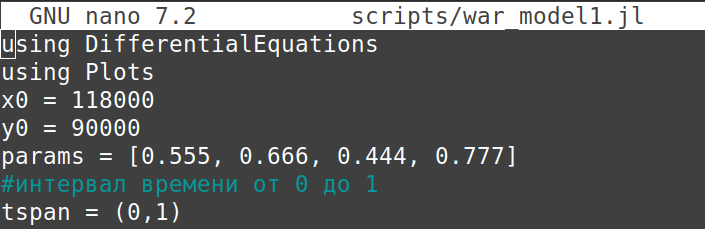
\includegraphics[width=0.7\textwidth,height=\textheight]{image/pic11.png}

}

\caption{\label{fig-001}Присвоение значений}

\end{figure}%

Функция, описывающая подход первого подкрепления армии, θ(θ) = 2cos(t),
второе подкрепление армии описывается функцией θ(θ) = 2sin(t). Затем
получаем систему, описывающую противостояние регулярных войск 𝑋 и 𝑌. Я
записываю систему ODE с помощью функции, задаю соответствующую задачу
Коши с помощью ODEProblem и решаю ее с помощью solve, затем строю график
решения(рис.2)

\begin{figure}

\centering{

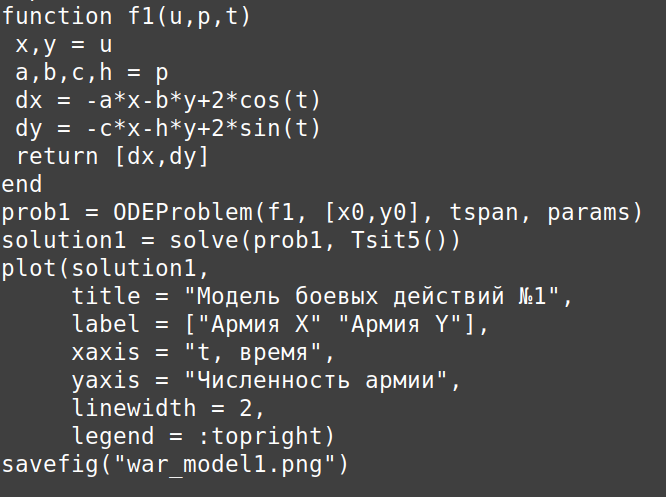
\includegraphics[width=0.7\textwidth,height=\textheight]{image/pic12.png}

}

\caption{\label{fig-002}Функции}

\end{figure}%

В результате мы видим, что при таких параметрах модели армия X
побеждает(рис.3)

\begin{figure}

\centering{

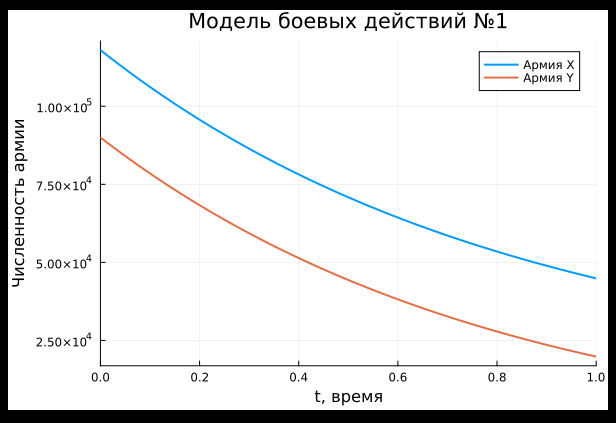
\includegraphics[width=0.7\textwidth,height=\textheight]{image/pic3.png}

}

\caption{\label{fig-003}Результат}

\end{figure}%

\subsection{Реализация в
scilab}\label{ux440ux435ux430ux43bux438ux437ux430ux446ux438ux44f-ux432-scilab}

Я создаю ту же модель, используя scilab. Модель определяется следующим
образом:

\begin{verbatim}
x0 = 118000;
y0 = 90000;
t0 = 0;

a = 0.555;
b = 0.666;
c = 0.444;
h = 0.777;

tmax = 1;

dt = 0.01;

t = [t0:dt:tmax];

function p = P(t)
p = 2*cos(t);
endfunction

function q = Q(t)
q = 2*sin(t);
endfunction

function dy = syst(t,y)
dy(1) = -a*y(1)-b*y(2)+P(t);
dy(2) = -c*y(1)-h*y(2)+Q(t);
endfunction

v0 = [x0;y0];

y = ode(v0,t0,t,syst);

scf(0);
plot2d(t,y(1,:),style=2);
xtitle("Модель боевых действий № 1", "Шаг", "Численность армии");
plot2d(t,y(2,:), style=5);
xgrid();
\end{verbatim}

Мы видим, что график совпадает с тем, который мы получили с помощью
Julia, никакой разницы(рис.4)

\begin{figure}

\centering{

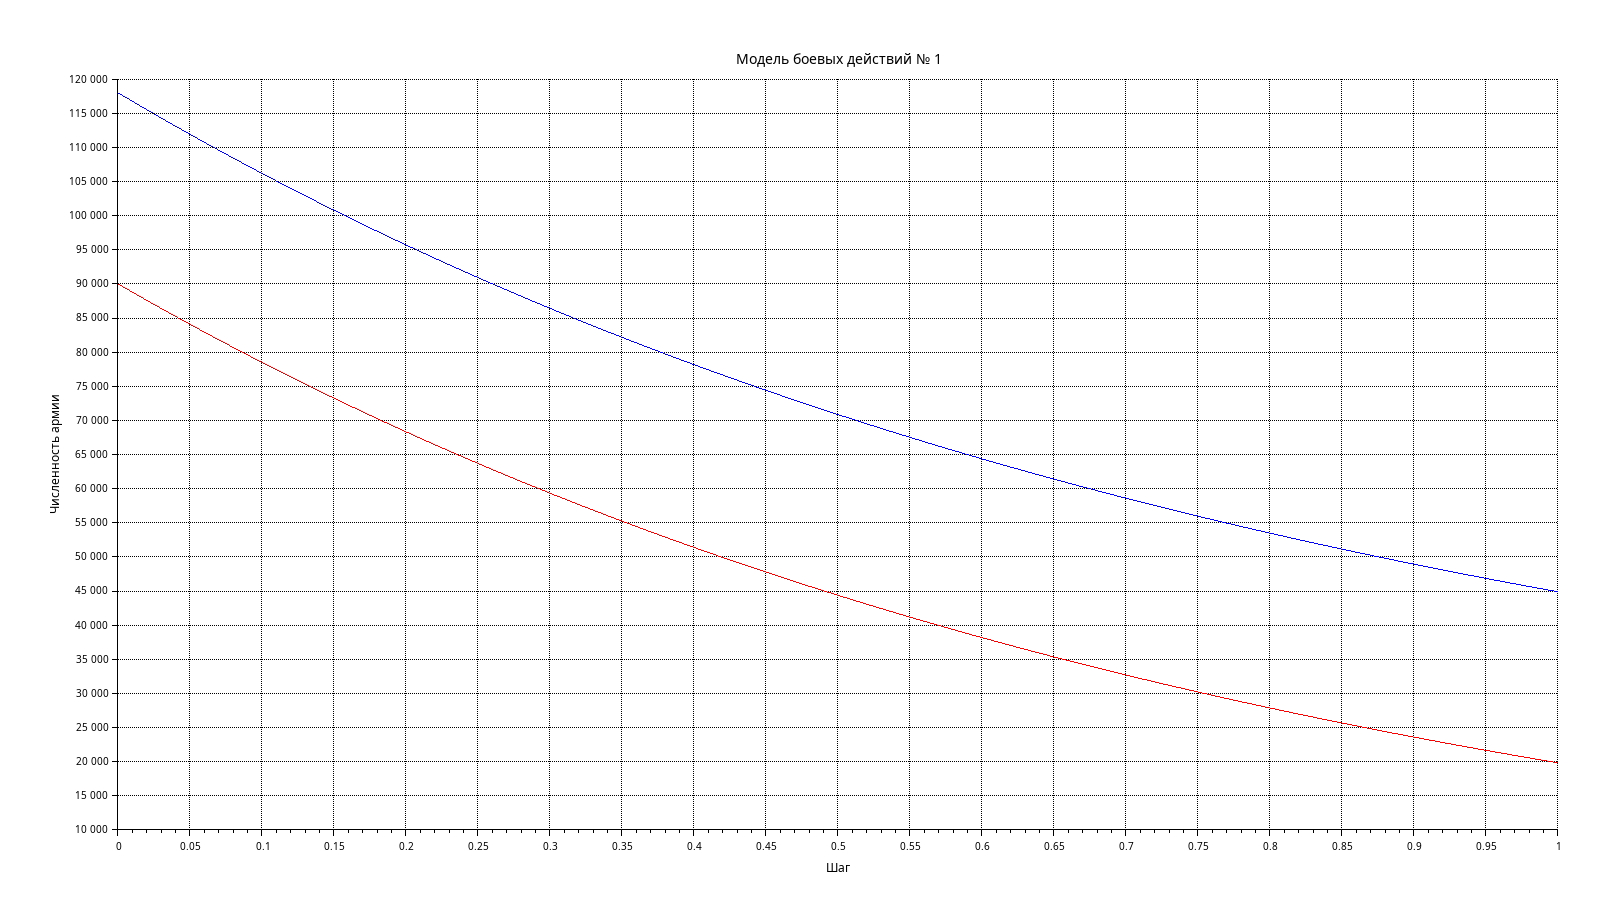
\includegraphics[width=0.7\textwidth,height=\textheight]{image/pic5.png}

}

\caption{\label{fig-004}Результат}

\end{figure}%

\section{Модель ведение боевых действий с участием регулярных войск и
партизанских
отрядов}\label{ux43cux43eux434ux435ux43bux44c-ux432ux435ux434ux435ux43dux438ux435-ux431ux43eux435ux432ux44bux445-ux434ux435ux439ux441ux442ux432ux438ux439-ux441-ux443ux447ux430ux441ux442ux438ux435ux43c-ux440ux435ux433ux443ux43bux44fux440ux43dux44bux445-ux432ux43eux439ux441ux43a-ux438-ux43fux430ux440ux442ux438ux437ux430ux43dux441ux43aux438ux445-ux43eux442ux440ux44fux434ux43eux432}

\subsection{Реализация в
Julia}\label{ux440ux435ux430ux43bux438ux437ux430ux446ux438ux44f-ux432-julia-1}

Модель боевых действий между регулярными войсками. Я присваиваю значения
коэффициенту смертности, который не связан с боевыми операциями, и
коэффициентам эффективности первой и второй армий. Значения приведены в
задаче(рис.5).

\begin{figure}

\centering{

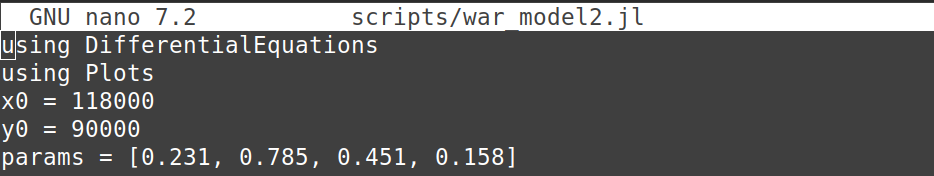
\includegraphics[width=0.7\textwidth,height=\textheight]{image/pic13.png}

}

\caption{\label{fig-005}Присвоение значений}

\end{figure}%

Функция, описывающая подход первого подкрепления армии, θ(θ) = cos(2t),
второе подкрепление армии описывается функцией θ(θ) = sin(3t). Затем
получаем систему, описывающую противостояние регулярных войск 𝑋 и 𝑌. Я
записываю систему ODE с помощью функции, задаю соответствующую задачу
Коши с помощью ODEProblem и решаю ее с помощью solve, затем строю график
решения(рис.6)

\begin{figure}

\centering{

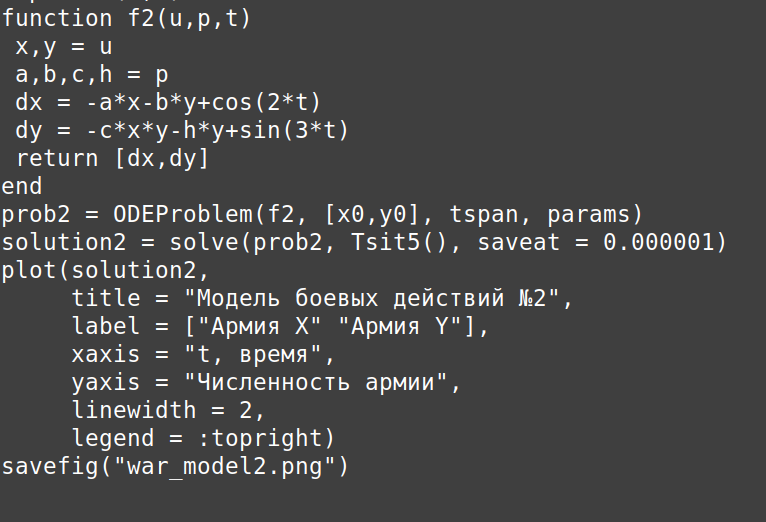
\includegraphics[width=0.7\textwidth,height=\textheight]{image/pic16.png}

}

\caption{\label{fig-006}Функции}

\end{figure}%

В результате мы видим, что при таких параметрах модели армия X побеждает
за короткий промежуток времени(рис.7)

\begin{figure}

\centering{

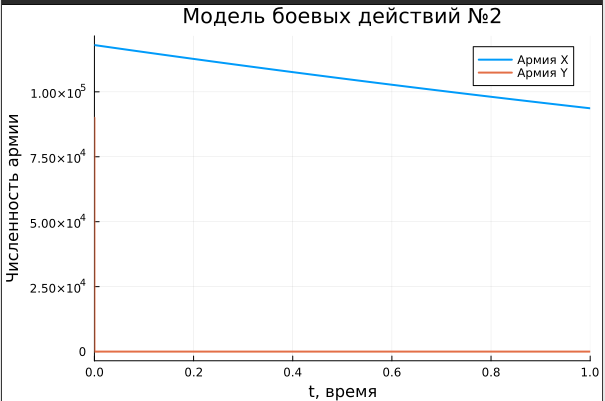
\includegraphics[width=0.7\textwidth,height=\textheight]{image/pic15.png}

}

\caption{\label{fig-007}Результат}

\end{figure}%

\subsection{Реализация в
scilab}\label{ux440ux435ux430ux43bux438ux437ux430ux446ux438ux44f-ux432-scilab-1}

Я создаю ту же модель, используя scilab. Модель определяется следующим
образом:

\begin{verbatim}
x0 = 118000;
y0 = 90000;
t0 = 0;

a = 0.231;
b = 0.785;
c = 0.451;
h = 0.158;

tmax = 1;

dt = 0.000001;

t = [t0:dt:tmax];

function p = P(t)
p = cos(2*t);
endfunction

function q = Q(t)
q = sin(3*t);
endfunction

function dy = syst(t,y)
dy(1) = -a*y(1)-b*y(2)+P(t);
dy(2) = -c*y(1)*y(2)-h*y(2)+Q(t);
endfunction

v0 = [x0;y0];

y = ode(v0,t0,t,syst);

scf(0);
clf();
plot2d(t, y(1,:), style=2, rect=[0, 0, 0.0002, 40000]);
plot2d(t, y(2,:), style=5, rect=[0, 0, 0.0002, 40000]);
xtitle("Модель боевых действий № 1", "Шаг", "Численность армии");
xgrid();
\end{verbatim}

Мы видим, что график совпадает с тем, который мы получили с помощью
Julia, никакой разницы(рис.8)

\begin{figure}

\centering{

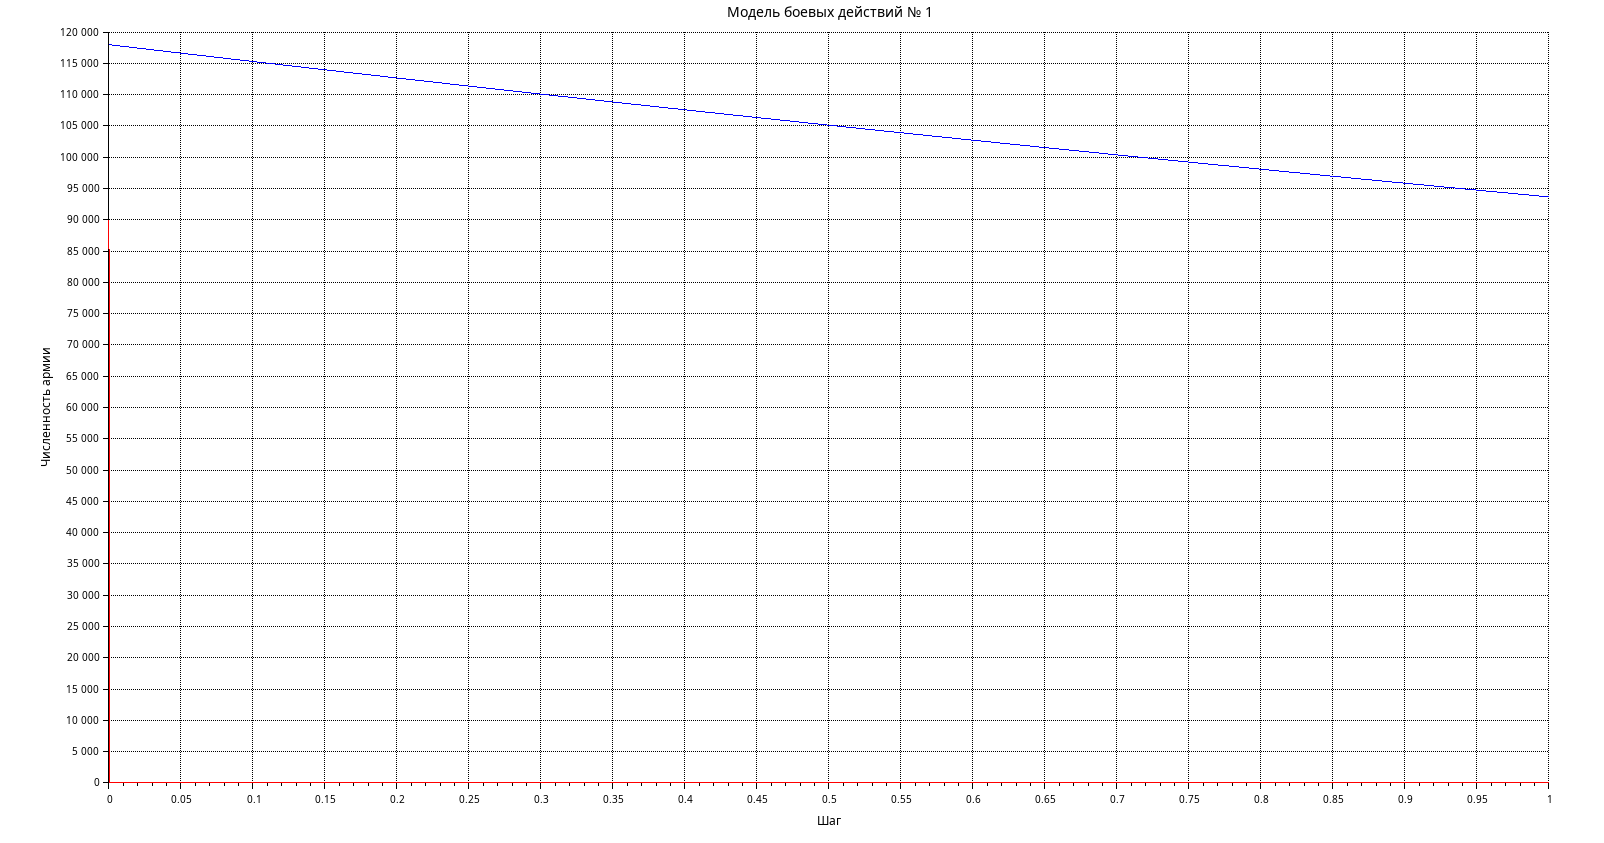
\includegraphics[width=0.7\textwidth,height=\textheight]{image/pic9.png}

}

\caption{\label{fig-008}Результат}

\end{figure}%

Чтобы ясно видеть, как уменьшается количество солдат армии Y, я
установила пределы x и y от 0,0002 до 40000(рис.9)

\begin{figure}

\centering{

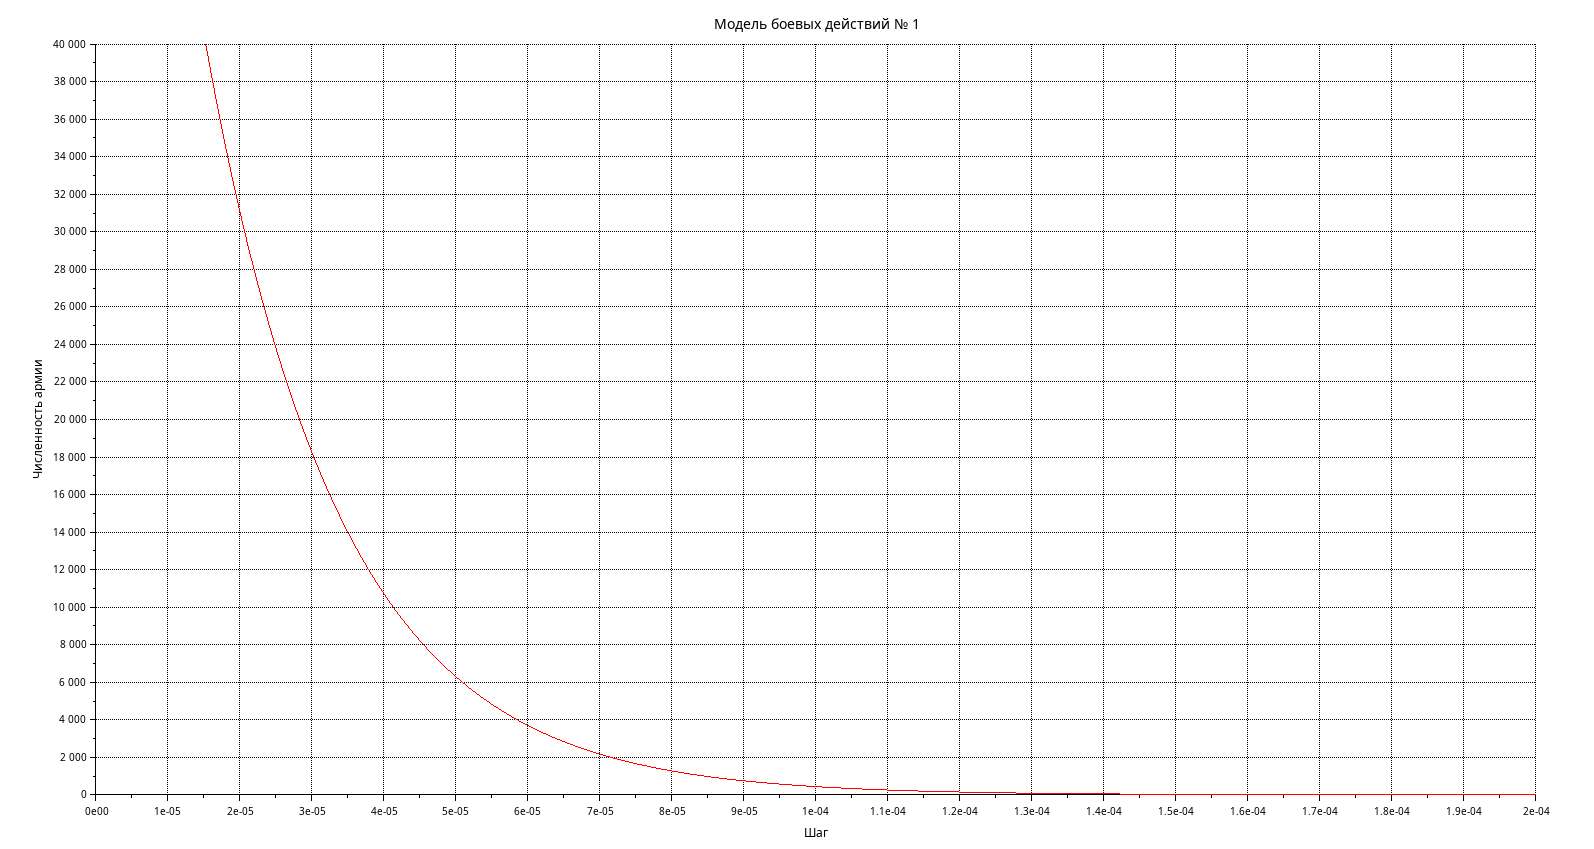
\includegraphics[width=0.7\textwidth,height=\textheight]{image/pic10.png}

}

\caption{\label{fig-009}Результат}

\end{figure}%

\chapter{Выводы}\label{ux432ux44bux432ux43eux434ux44b}

В этой лабораторной работе я построила математическую модель боевых
действий.


\printbibliography


\end{document}
